\section{W7: Formal SDLC Project Scheduling}

\textbf{1. Formal SDLC Project Schedule.}

\textbf{3. Developing Project Schedule - Steps.}

    \textbf{3.1. Breakdown the task into small chunks you can deal with – Work Breakdown Structure (WBS).}

        \textbf{3.1.1. Fishbone Diagram.}
        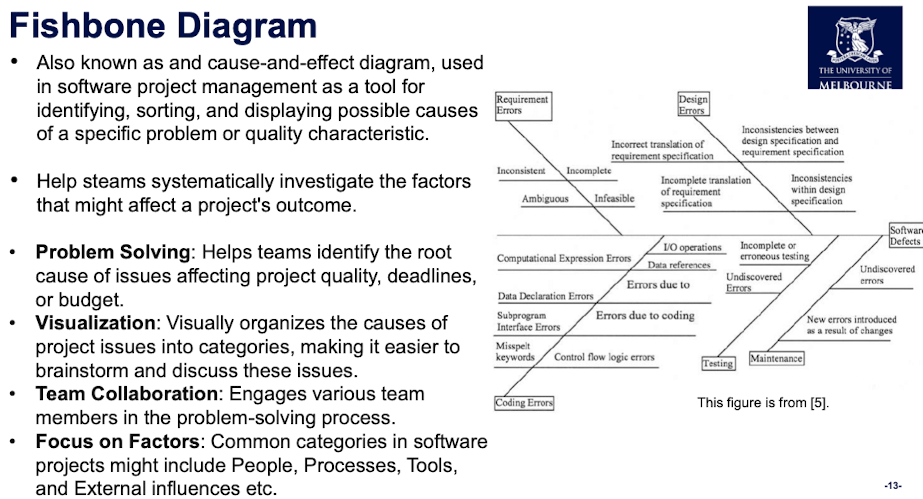
\includegraphics[width=\linewidth]{figs/SCR-20240606-oxhd.png}

    \textbf{3.2. Identify the interdependencies between the broken-down tasks and develop a task network.}
    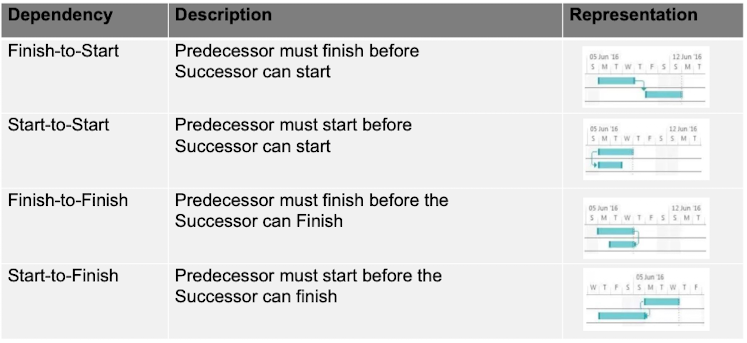
\includegraphics[width=\linewidth]{figs/SCR-20240606-oyge.png}

    \textbf{3.3. Estimate the effort and the time allocation for each task.}
    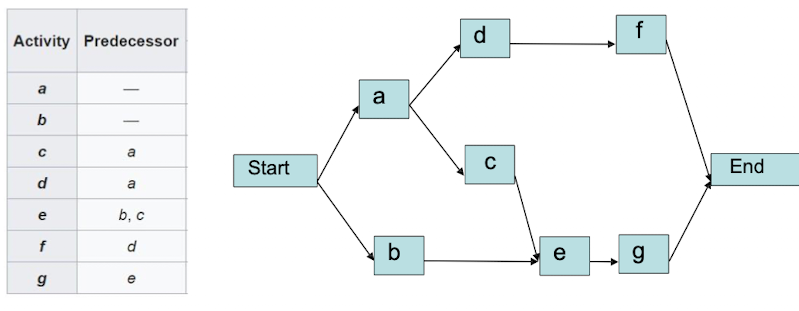
\includegraphics[width=\linewidth]{figs/SCR-20240606-oyqc.png}

        \textbf{3.3.1. Putnam-Norden-Rayleigh (PNR) curve.}
        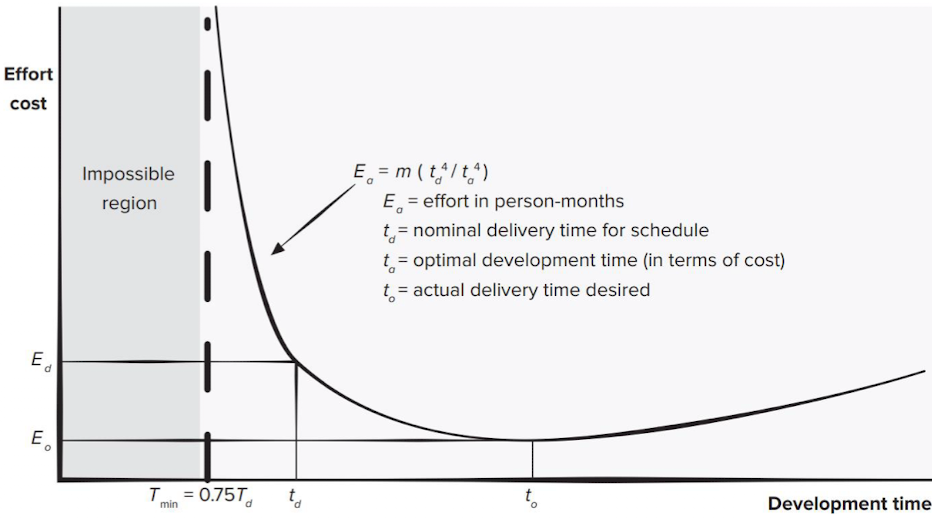
\includegraphics[width=\linewidth]{figs/SCR-20240606-ozjp.png}
        The PNR curve indicates the project delivery time cannot be compressed much beyond $0.75t_d$. It also indicates that the lowest cost delivery option $t_o = 2t_d$. The implication here is that delaying project delivery can reduce costs significantly.

        \textbf{3.3.2. Three-Point Estimating:} technique used in project management to estimate the duration or cost of a task with a more refined approach than a single-point estimate. It considers uncertainty and the risk of potential variation in task estimates. Optimistic time (O), pessimistic time (P), most likely time (M).

            \textbf{3.3.2.1. Triangular Distribution.}
            The expected time (TE) is calculated as $T_E = (O + M + P) / 3$.

            \textbf{3.3.2.2. PERT Distribution.}
            Most likely scenario is weighted more heavily. $T_E = (O + 4M + P) / 6$.

    \textbf{3.4. Allocate resources for tasks and validate effort.}


    \textbf{3.5. Develop the project schedule}: Two widely used techniques are Gantt Chart and PERT Chart.

        \textbf{3.5.1. Gantt Chart}: linked Gantt chart and progress Gantt chart
        % 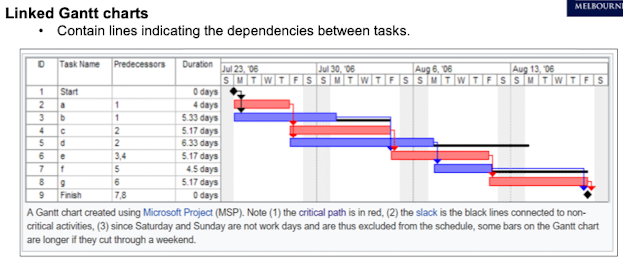
\includegraphics[width=\linewidth]{figs/SCR-20240606-pfel.png}
        % 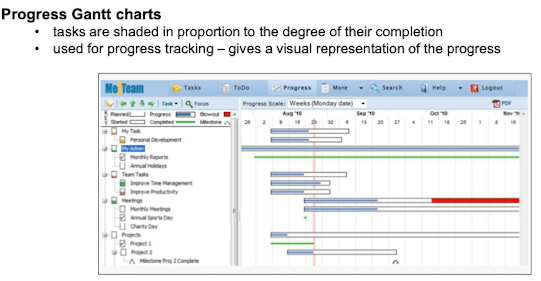
\includegraphics[width=\linewidth]{figs/SCR-20240606-pffv.png}

        \textbf{3.5.2. PERT Chart}: Program Evaluation and Review Technique chart, a task network which shows the dependencies along with time related information and the critical path.
        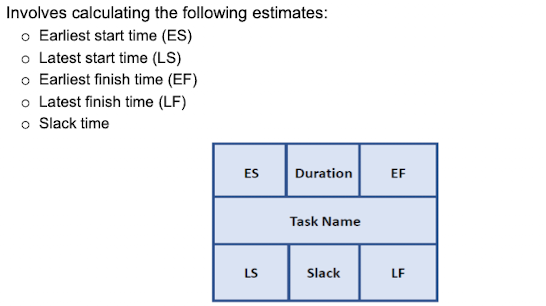
\includegraphics[width=\linewidth]{figs/SCR-20240606-pfyr.png}
        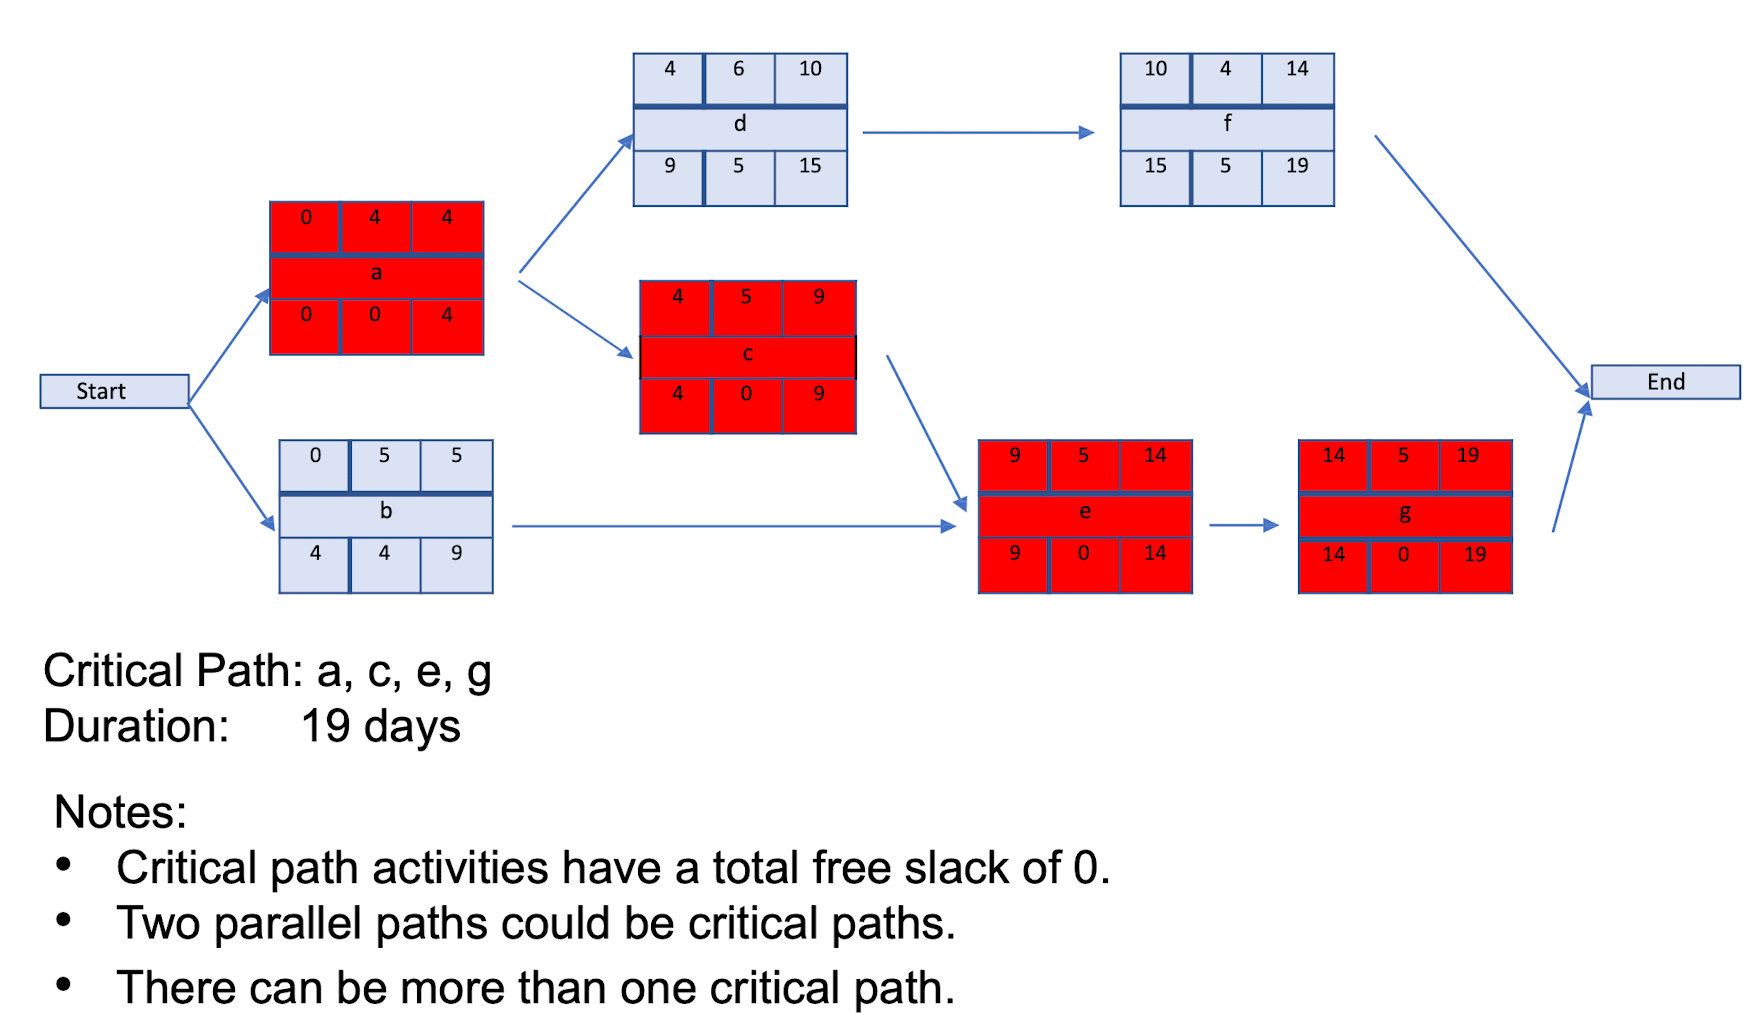
\includegraphics[width=\linewidth]{figs/SCR-20240606-pggc.png}

\textbf{7. Project Tracking and Control.}

    \textbf{7.1. Earned Value Analysis}: Planned value (PV) that portion of the approved cost estimate planned to be spent on the given activity during a given period. Earned Value (EV) the value of the work actually completed. Actual Cost (AC) the total of the costs incurred in accomplishing work on the activity in a given time period.
    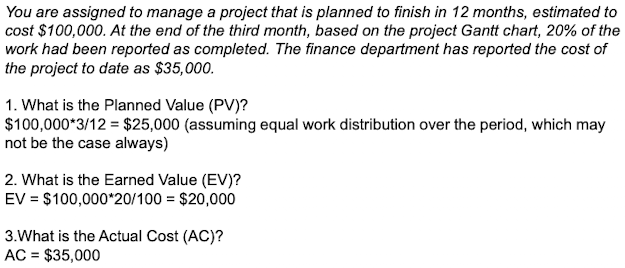
\includegraphics[width=\linewidth]{figs/SCR-20240606-pidd.png}

    \textbf{7.2. Schedule Variance Analysis.}
    
    SV = EV - PV. If SV greater than 0, project is ahead of schedule. If SV less than 0, project is behind schedule. SPI (schedule performance index) = EV / PV. If SPI greater than 1, project is ahead of schedule. If SPI less than 1, project is behind schedule.

    \textbf{7.3. Cost Variance Analysis.}
    CV = EV - AC. If CV greater than 0, project is under budget. If CV less than 0, project is over budget. CPI (cost performance index) = EV / AC.
    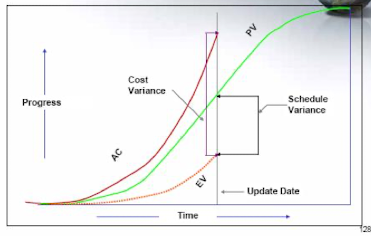
\includegraphics[width=\linewidth]{figs/SCR-20240606-pjgq.png}